\documentclass{article}
\usepackage{amsmath}
\usepackage{amsfonts}
\usepackage{amssymb}
\usepackage{libs/commath2}
\usepackage[table]{xcolor}
\usepackage[hidelinks,draft=false]{hyperref}
\usepackage[skins,theorems]{tcolorbox}
\usepackage{titlesec}
\usepackage{tikz}
\usepackage{libs/circuitikz} % use our own recent version to make sure some bugs are fixed
\usepackage{pgfplots}
\usepackage{mathtools}
\usepackage[makeroom]{cancel}
\usepackage{mathrsfs}
\usepackage{wrapfig}
%\usepackage{subcaption}
%\usepackage{floatrow}
\usepackage{esint}
\usepackage{paralist}
\usepackage{enumitem}
%\usepackage{bm}
\usepackage{relsize}
\usepackage{xfrac}
\usepackage{comment}
\usepackage{siunitx}
\usepackage{multicol}
%\usepackage{MnSymbol}
\usepackage[obeyDraft,textsize=tiny]{todonotes}
%\usepackage{morefloats} % oh no!
%\usepackage[linesnumbered,lined]{algorithm2e}
\usepackage{glossaries}
\usepackage{xifthen}
\usepackage{tocloft}
\usepackage{nccmath}


\pgfplotsset{compat=1.13}
\usetikzlibrary{arrows.meta}
\usetikzlibrary{patterns}
\usetikzlibrary{decorations.pathmorphing}
\usetikzlibrary{decorations.markings}
\usetikzlibrary{backgrounds}
\usetikzlibrary{shapes.misc}
\usetikzlibrary{shapes.multipart}
\usetikzlibrary{shadows.blur}
\usetikzlibrary{fadings}
\usetikzlibrary{intersections}
\usetikzlibrary{arrows.meta}
\usetikzlibrary{calc}
\usetikzlibrary{matrix}
\usetikzlibrary{positioning}
\usetikzlibrary{shapes}
\usetikzlibrary{shadings}

\tcbuselibrary{breakable}
\tcbuselibrary{skins}
\tcbuselibrary{xparse}

\tikzset{cross/.style={cross out, draw,
        minimum size=2*(#1-\pgflinewidth),
        inner sep=0pt, outer sep=0pt}}
\tikzset{
    mark position/.style args={#1(#2)}{
        postaction={
            decorate,
            decoration={
            	post length=1mm, % ??? Magic to fix "Dimension
            	pre length=1mm, % ???  too large" errors.
                markings,
                mark=at position #1 with \coordinate (#2);
            }
        }
    }
}
\tikzset{
	arrow at/.style args={#1}{
		postaction={
			decorate,
			decoration={
				post length=1mm, % ??? Magic to fix "Dimension
				pre length=1mm, % ???  too large" errors.
				markings,
				mark=at position #1 with {\arrow{>}};
			}
		}
	}
}
\makeatletter
\tikzset{
  use path for main/.code={%
    \tikz@addmode{%
      \expandafter\pgfsyssoftpath@setcurrentpath\csname tikz@intersect@path@name@#1\endcsname
    }%
  },
  use path for actions/.code={%
    \expandafter\def\expandafter\tikz@preactions\expandafter{\tikz@preactions\expandafter\let\expandafter\tikz@actions@path\csname tikz@intersect@path@name@#1\endcsname}%
  },
  use path/.style={%
    use path for main=#1,
    use path for actions=#1,
  }
}
\makeatother

\pgfmathdeclarefunction{sinc}{1}{%
	\pgfmathparse{abs(#1)<0.01 ? int(1) : int(0)}%
	\ifnum\pgfmathresult>0 \pgfmathparse{1}\else\pgfmathparse{sin(#1 r)/#1}\fi%
}
\pgfmathdeclarefunction{gauss}{2}{%
	\pgfmathparse{1/(#2*sqrt(2*pi))*exp(-((x-#1)^2)/(2*#2^2))}%
}

\usepackage[left=2cm,right=2cm,top=2cm,bottom=2cm]{geometry}

%\usepackage[no-math]{fontspec}
%\usepackage{fontspec}
\usepackage{mathspec}
%\usepackage{newtxtext,newtxmath}
%\usepackage{unicode-math}
%\setmainfont{texgyretermes-regular.otf}
%\setsansfont{texgyreheros-regular.otf}
%\newfontfamily\greekfont[Script=Greek]{Linux Libertine O}
%\newfontfamily\greekfontsf[Script=Greek]{Linux Libertine O}
\usepackage{polyglossia}
%\newfontfamily\greekfont[Script=Greek]{texgyretermes-regular.otf}
\newfontfamily\greekfontsf[Script=Greek]{texgyreheros-regular.otf}
\newfontfamily\greekfonttt[Script=Greek]{Latin Modern Mono}
%\usepackage[greek]{babel}
\setdefaultlanguage{greek}
\setotherlanguage{english}

%\usepackage[utf8]{inputenc}
%\usepackage[greek]{babel}


%\usepackage{tkz-euclide} % loads  TikZ and tkz-base
%\usetkzobj{angles} % important you want to use angles

\newlist{enumparen}{enumerate}{1}
\setlist[enumparen]{label=(\arabic*)}
\newlist{enumpar}{enumerate}{1}
\setlist[enumpar]{label=\arabic*)}

\newlist{enumgreek}{enumerate}{1}
\setlist[enumgreek]{label=\alph*.}
\newlist{enumgreekparen}{enumerate}{1}
\setlist[enumgreekparen]{label=(\alph*)}
\newlist{enumgreekpar}{enumerate}{1}
\setlist[enumgreekpar]{label=\alph*)}


\newlist{enumroman}{enumerate}{1}
\setlist[enumroman]{label=(\roman*)}

\newlist{enumlatin}{enumerate}{1}
\setlist[enumlatin]{label=(\alph*)}

\newlist{invitemize}{itemize}{1}
\setlist[invitemize]{noitemsep,label=}

\input{libs/fiximplies}
%\input{libs/sphere}

\makeatletter
\let\anw@true\anw@false

%\newcommand{\attnboxed}[1]{\textcolor{red}{\fbox{\normalcolor\m@th$\displaystyle#1$}}}
\makeatother
\tcbset{highlight math style={enhanced,colframe=red,colback=white,%
        arc=0pt,boxrule=1pt,shrink tight,boxsep=1.5mm,extrude by=0.5mm}}
\newcommand{\attnboxed}[1]{\tcbhighmath[colback=red!5!white,drop fuzzy shadow,arc=0mm]{#1}}
\newcommand{\infoboxed}[1]{%
	\tcbhighmath[colframe=blue!50!white,colback=blue!5!white,arc=0mm]{#1}}
\titleformat{\section}{\bf\Large}{Κεφάλαιο \thesection}{1em}{}
\newtcolorbox{attnbox}[1]{colback=red!5!white,%
    colframe=red!75!black,fonttitle=\bfseries,title=#1}
\newtcbox{quickattnbox}[1]{colback=red!5!white,%
	colframe=red!75!black,fonttitle=\bfseries,title=#1}
\newtcolorbox{infobox}[1]{colback=blue!5!white,%
    colframe=blue!75!black,fonttitle=\bfseries,title=#1}
\newtcolorbox{knowledgebox}[2][]{colbacktitle=red!10!white,
	colback=blue!10!white,coltitle=blue!70!black,
	attach title to upper,after title={:\ },
	title={#2},fonttitle=\bfseries,#1}
%TODO: Knowledge titles to left
\newtcolorbox{questionbox}[2][]{
beamer,title={#2},#1}

\tcbset{frogbox/.style={enhanced jigsaw,%
		overlay first={\foreach \x in {0cm} {
				\begin{scope}[shift={([xshift=-0.2cm]title.west)}]
					\draw[very thick,green!65!black!50!white,latex-] (0,0) -- ++(-1.5,0);
\end{scope}}}}}
\tcbset{frogtitle/.style={
attach boxed title to top left=
{xshift=0mm,yshift=-0.50mm},
boxed title style={skin=enhancedfirst jigsaw,
	bottom=0mm,
	interior style={fill=none,
		left color=green!20!black,
		right color=gray}}
}}
\DeclareTColorBox{exercise}{ O{} }{
	enhanced jigsaw,
	breakable,parbox=false,
	%title style={left color=gray!50!white!50!green,opacity=.5,right color=white},
	subtitle style={%boxrule=1pt,
		colback=yellow!50!red!25!white,fontupper=\bfseries},
	coltitle=black,colbacktitle=blue!90!black!25!white,colframe=black,
	frame hidden,
	boxrule=0mm,
	%boxrule=1mm,
	leftrule=0.8pt,toprule=0.8pt,rightrule=0pt, %reserve space
	borderline west={0.8pt}{0pt}{white!25!black},%---- draw line
	borderline north={0.8pt}{0pt}{white!25!black},%---- draw line
	interior hidden,
	%frame style={left color=black,right color=white},
	sharp corners=all,
	%frogbox, %TODO: frogbox
	before lower={\tcbsubtitle[before skip=\baselineskip]{Λύση}},lower separated=false,
	before title={\textbf{Άσκηση\ifthenelse{\isempty{#1}}{}{: }}},
	title={\ifthenelse{\isempty{#1}}{\hspace{0pt}}{#1}}%
}

% Minipage utilities
\newcommand{\saveparinfo}{%
	\edef\myindent{\the\parindent}%
	\edef\myparskip{\the\parskip}}

\newcommand{\useparinfo}{%
	\setlength{\parindent}{\myindent}%
	\setlength{\parskip}{\myparskip}}

\AtBeginDocument{%
\let\arg\relax
\let\Re\relax
\let\Im\relax
\DeclareMathOperator{\arg}{arg}
\DeclareMathOperator{\Re}{Re}
\DeclareMathOperator{\Im}{Im}
}
\DeclareMathOperator{\sinc}{sinc}
\DeclareMathOperator{\sgn}{sgn}
\DeclareMathOperator{\erf}{erf}
\DeclareMathOperator{\cov}{cov}
\DeclareMathOperator{\atand}{atan2}
\DeclareMathOperator{\rank}{rank}
\DeclareMathOperator{\res}{Res}

\newenvironment{absolutelynopagebreak}
{\par\nobreak\vfil\penalty0\vfilneg
	\vtop\bgroup}
{\par\xdef\tpd{\the\prevdepth}\egroup
	\prevdepth=\tpd}

\DeclareSIUnit \voltampere { VA } %apparent power 
\DeclareSIUnit \var { VAr } %volt-ampere reactive - idle power 
\DeclareSIUnit \decade { dec } %decade

% Link colours
\hypersetup{colorlinks,linkcolor={blue!40!black!95!green},citecolor={blue!50!black},urlcolor={cyan!70!black}}

% Global amount of samples
% Set to a higher value (e.g. 200) for nicer graphs
% Set to a low value (e.g. 10) for performance
% NOTE: Check the sample variables below for further measurements
\newcommand*{\gsamples}{200}

% Equals command as a workaround for CircuiTikZ bug
% not allowing the = sign in labels
\newcommand*{\equals}{=}

\newcommand{\nesearrow}{%
	\,%
	\smash{\raisebox{-1.1ex}
		{$%
			\stackrel{\displaystyle\nearrow}{\displaystyle\searrow}%
			$}}%
}
\newcommand{\degree}{^{\circ}} % not great
\newcommand\numberthis{\addtocounter{equation}{1}\tag{\theequation}} % add an equation number to a number-less math environment

% Provided commands
\providecommand\dif{d}
\providecommand\od[2]{\frac{#1}{#2}}

\newtcbtheorem[number within=section,list inside=thm]{theorem}{Θεώρημα}%
{colback=green!5,colframe=green!35!black,colbacktitle=green!35!black,fonttitle=\bfseries,enhanced,attach boxed title to top left={yshift=-2mm,xshift=-7mm},width=.9\textwidth,arc=.7mm}{th}
\newtcbtheorem[number within=section,list inside=defn]{defn}{Ορισμός}%
{colback=blue!5,colframe=cyan!35!black,colbacktitle=blue!35!black,fonttitle=\bfseries,enhanced,attach boxed title to top left={yshift=-2mm,xshift=-2mm}}{def}

\makeatletter
\def\tcb@cnt@theoremautorefname{Θεώρημα}
\def\tcb@cnt@defnautorefname{Ορισμός}
\makeatother

% Locus plot utilities
\tikzset{locus/.style={orange!50!red!70!brown}}
\tikzset{locuspole/.style={draw=red!30!black,cross,inner sep=2.5pt,fill=white,fill opacity=.6,thick,label={[below]-90:#1}}}
\tikzset{locuszero/.style={draw=red!30!black,circle,inner sep=2pt,fill=white,fill opacity=.6,thick,label={[below]-90:#1}}}
\tikzset{locusbreak/.style={rounded corners=1.5pt,inner sep=2pt,draw,top color=brown,bottom color=black,fill opacity=.8,label={[below]-90:#1}}}

% Lecture specifications

\newcommand{\listlecturename}{Κατάλογος Διαλέξεων}
\newlistof[chapter]{lecture}{toclec}{\listlecturename}
\renewcommand{\cfttoclectitlefont}{\normalfont\Large\bfseries}

\newcommand{\lecture}[2]{%
	\refstepcounter{lecture}
	\addcontentsline{toclec}{lecture}{\protect\numberline{#1}Διάλεξη #2}
	\hypertarget{lecture_#1}{}
	\nointerlineskip \vspace{.4\baselineskip}%\hspace{\fill}
	\centerline{%\color{#1}
		%\resizebox{1.1\linewidth}{\height}
		\smash{{%
				{\begin{tikzpicture}[xscale=2,baseline={([yshift=0ex]current bounding box.north)}]
					\draw[blue!50!cyan,path fading=west] (0,0) -- (10.1,0);
					\draw[blue!60!cyan!30!white,path fading=east] (0,0) -- (10.1,0);
					\draw[>-,blue!60!cyan!70!white,>={LaTeX[scale=2]},draw opacity=1] (9.9,0) -- ++(0,-0.01);
					\draw (9.9,-0.4) node[rectangle,align=center,scale=.7,blue!70!black,below]
					{Διάλεξη #1\textsuperscript{η}\\#2};
					\end{tikzpicture}}}}}%
	%\hspace{\fill}
	\par\nointerlineskip \vspace{.5\baselineskip}
}

%\newcommand{\autopageref}[1]{%
%\hyperref[#1]{Σελίδα \pageref*{#1}}%
%}

% Note: Latex requires a configuration flag for PDF named destinations to be stored:
% In dvipdfmx.cfg search for Dvipdfmx Compatibility Flags, and add this line after %C  0x0000:
%     C  0x0010
%

% New plotting utilities
\def\vlowsamples{4}
\def\lowsamples{40}
\def\midsamples{60}
\def\hisamples{80}
\def\timecolour{blue!50!cyan!80!brown}
\def\omegacolour{red!50!orange!90!brown}

\tikzstyle{timecolour}=[\timecolour]
\tikzstyle{omegacolour}=[\omegacolour]

\renewcommand*{\pageautorefname}{Σελίδα}
\renewcommand*{\sectionautorefname}{Ενότητα}
\renewcommand*{\subsectionautorefname}{Ενότητα}
\renewcommand*{\subsubsectionautorefname}{Ενότητα}


\usepackage{pdfpages}


%%%%%%%%%%%%%%%%%%%%%%%%%%%%%%%%%%%%%%%%%%%%%%%%%%%%%%%%%%%%%%%%%%%%
\title{\vspace{1.2cm}\textbf{Βοήθημα Έδρανων Ολίσθησης }}
\date{\textbf{\today}}
\author{Για τον κώδικα σε \LaTeX, ενημερώσεις και προτάσεις:\\ \small\url{https://github.com/PavlosRakovalis/MengNotes/tree/main/Stoiheia1/Έδρανα_Κυλίσεως_Βοήθημα}}
%%%%%%%%%%%%%%%%%%%%%%%%%%%%%%%%%%%%%%%%%%%%%%%%%%%%%%%%%%%%%%%%%%%%





%document starts here, who would have imagined that?
\begin{document}
%set AERONAUTICS_REPORT_TEMPLATE as template JUST for this page
%the asterisk means it will be set just for this page
\AddToShipoutPicture*{\BackgroundPic}
 \maketitle
\maketitle
%leave a bunch of empty space for the contents
\vspace{6cm}
%shows contents automatically. Every section, subsection, etc automatically shows up here
\tableofcontents{}
%change page
\pagebreak
%create new command about pics on all other pages
\ClearShipoutPicture
\newcommand\Bgpic{
    \put(-4,0){
    \parbox[b][\paperheight]{\paperwidth}{%
    \vfill
    \centering
    
\includegraphics[width=\paperwidth,height=\paperheight]{AERONAUTICS_REPORT_TEMPLATE-pages-2.pdf}
    \vfill
    }}}
%set background picture for every page after page 2, including page 2
%see, no asterisk
\AddToShipoutPicture{\Bgpic}
%yay, our first section, who would have thought




%%%%%%%%%%%%%%%%%%%%%%%%%%%%%%%%%%%%%%%%%%%%%%%%%%%%%%%%%%%%%%%%%
%%%%%%%%%%%%%%%%%%%%%%%%%%%%%%%%%%%%%%%%%%%%%%%%%%%%%%%%%%%%%%%%%
%%%%%%%%%%%%%%%%%%%%%%%%%%%%%%%%%%%%%%%%%%%%%%%%%%%%%%%%%%%%%%%%%



%%%%%%%%%%%%%%%%%%%%%%%%%%%%%%%%%%%%%%%%%%%%%%%%%%%%%%%%%%%%%%%%%%%%%%%%%%%%
\section{Ονοματολογία συντελεστών}
\begin{itemize}
    \item $F_r$ ακτινική δύναμη που δέχεται το ρουλέμαν
    \item $F_d$ αξονική δύναμη που δέχεται το ρουλέμαν
    \item $n$ περιστροφική ταχύτητα του εδράνου σε rpm
    \item $L_h$ διάρκεια ζωής σε ώρες
    \item $P$ Ισοδύναμο φορτίο
    \item $C$ Αριθμός δυναμικής αντοχής
\end{itemize}


%%%%%%%%%%%%%%%%%%%%%%%%%%%%%%%%%%%%%%%%%%%%%%%%%%%%%%%%%%%%%%%%%%%%%%%%%%555555
\section{Εισαγωγή}
Στα έδρανα κυλήσεως μπορούμε να κάνουμε 2 υπολογισμόυς. Αυτοί είναι οι:
\begin{enumerate}   
    \item Υπολογισμός Μελέτης
    \item Υπολογισμό Αντοχής
\end{enumerate}
\\
Παρακάτω θα δούμε την μεθοδολογία του υπολογισμού Αντόχής




\section{Μεθοδολογία Υπολογισμού Μελέτης}
Για τον υπολογισμό μελέτης χρησιμοποιόυμε τον ίδιο τυπο που χρησημοποιόυμε στον υπολογισμό αντοχής, απλώς αντί να λύσουμε ως προς τον χρόνο που θα αντέξει το ρουλεμάν λύνουμε ώς πρός την δυναμική αντοχή.($C$) Για να το κάνουμε αυτό παίρνουμε σχετικά αυθαίρετες τιμές για $X$ και $Y$.Έπειτα με βάση αυτές τις τιμές βρίσκουμε ένα απαίτούμενο $C_α_π_α_ι_τ$. Έπειτα επιλέγουμε ένα ρουλεμάν το οποίο να ικανοποιεί το υπολογιζόμενο $C_α_π_α_ι_τ$. Επείτα κάνουμε υπολογισμό ελέγχου στο επιλεγμένο ρουλεμάν. Αν ο υπολογισμός ελέγχου μας δείξει οτι το ρουλεμάν μας δεν ικανοποιέι τις απαιτήσεις μας για αντοχή στον χρόνο τότε απλά επιλέγουμε ενα ρουλέμάν με μεγαλύτερο $C$ και επαναλαμβάνουμε τον υπολογισμό ελεγχου για να δούμε αν το δέυτερο ρουλεμάν ικανοποιέι τις απαιτήσεις μας για αντοχή στον χρόνο.


%%%%%%%%%%%%%%%%%%%%%%%%%%%%%%%%%%%%%%%%%%%%%%%%%%%%%%%%%%%%%%%%%%%%%%%%%%%%%%%%%%%
\section{ΔΕΣ,($F_r$ και $F_a$)}

\subsection{ΔΕΣ για απλά Ρουλεμάν}
Αρχικά πρέπει να βρώ τις δυνάμεις $F_r$ και $F_a$ μέσω Διαγράμματος Ελευθέρου σώμματος. Οι θέσεις και οι κατευθήνσεις των δυνάμεων είναι όπως είναι στο παρακάτω σχήμα.
%%%%%%%%%%%%%%%%%% na valw ena shima poy na veihnw katw apo pio simeio toy rouleman theoroyme oti askeitai i antidrasi
\\
\red{(!Προσοχή: Μόνο 1 απο τα 2 ρουλεμάν δέχεται την αξονική δύναμη)}
\\
Το έδρανο το οποίο δέχεται αξονική δύναμη συνήθως το ονομάζουμε έδρανο 1.
\\
\red{!Προσοχή: Είναι πολύ πιθανόν να χρειάζεται να κάνουμε ΔΕΣ τόσο στο επίπεδο XY όσο και στο επίπεδο ΧΖ.}(Πχ τα γρανάζια δέχονται και μία δύναμη ή οποία είναι επφαπτομένη στην περίμετρό τους και συνεπώς έιναι στο επίπεδο ΧΖ. Θέλει λοιπόν προσοχή στις δυνάμεις και στις ροπές.)


\subsection{ΔΕΣ για λοξά Ρουλεμάν}
Αρχικά μέσω Διαγράμματος Ελευθέρου σώμματος πρέπει να βρώ τις τιμές τών δυνάμεων στις θέσεις και τις κατευθύνσεις που βλέπουμε στο παρακάτω σχήμα.
\\
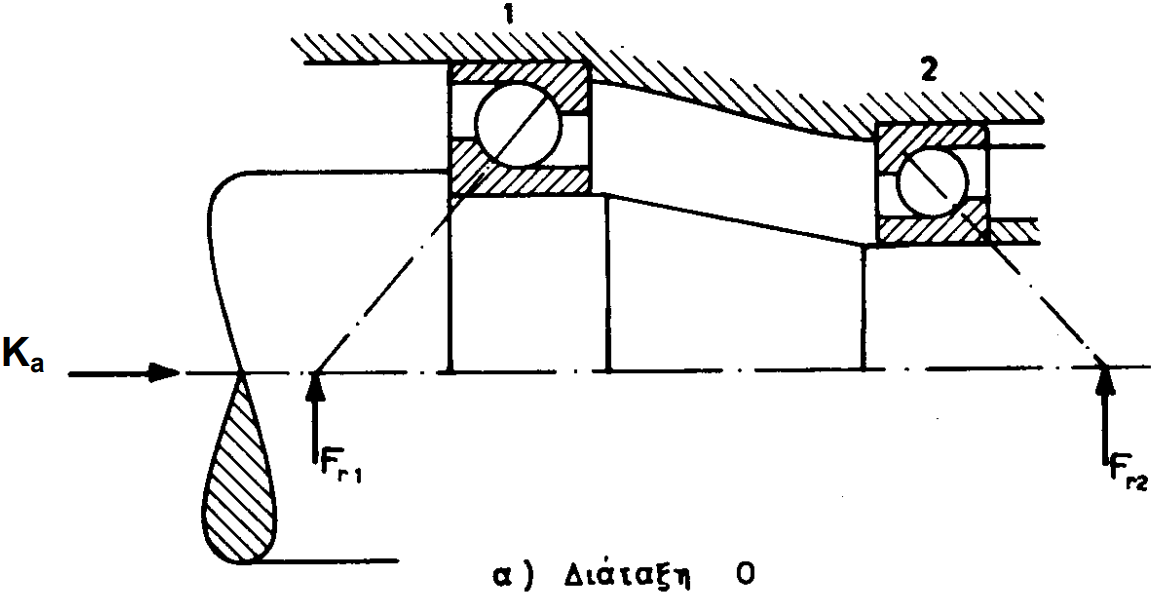
\includegraphics[width=0.5\linewidth]{3.png}
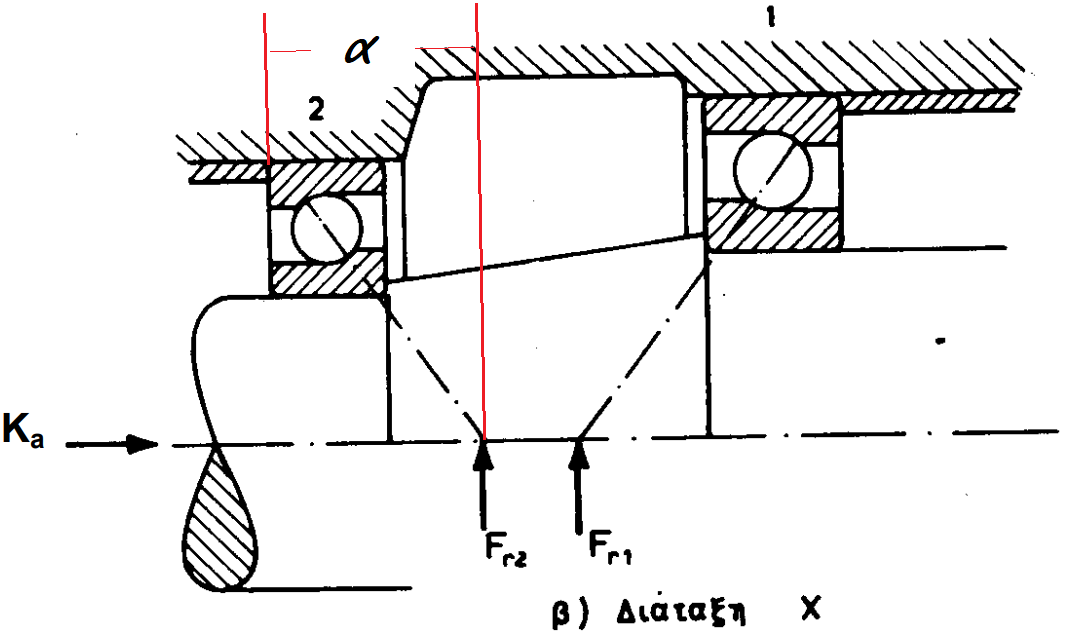
\includegraphics[width=0.5\linewidth]{3.1.png}
\\

\textbf{Η απόσταση α απο της αρχή του εδράνου στην οποία πρέπει να βρούμε την τιμή της ακτινικής δύναμης δίνεται ανάλογα με τον τύπο του ρουλεμάν απο τους πίνακες που βρίσκονται στο τέλος του pdf.} Το σημείο αυτό ονομάζεται κέντρο του κώνου πίεσης.
\\
\red{(!Προσοχή: Μόνο 1 απο τα 2 ρουλεμάν δέχεται την αξονική δύναμη)}
\\
Το έδρανο το οποίο δέχεται αξονική δύναμη συνήθως το ονομάζουμε έδρανο 1.
\\
\red{!Προσοχή: Είναι πολύ πιθανόν να χρειάζεται να κάνουμε ΔΕΣ τόσο στο επίπεδο XY όσο και στο επίπεδο ΧΖ.(Πχ τα γρανάζια δέχονται και μία δύναμη ή οποία είναι επφαπτομένη στην περίμετρό τους και συνεπώς έιναι στο επίπεδο ΧΖ. Θέλει λοιπόν προσοχή στις δυνάμεις και στις ροπές.}


%%%%%%%%%%%%%%%%%%%%%%%%%%%%%%%%%%%%%%%%%%%%%%%%%%%%%%%%%%%%%%%%%%%%%%%%%%%%%%%%%%%
\section{Δυνάμεις $F_r$ και $F_a$. \tiny{(kilopond)}}
Για να βρούμε τις δυνάμεις $F_r$ και $F_a$ υπάρχουν 2 πράγματα τα οποία πρέπει να προσέξουμε:
\\
\begin{itemize}
    \item \red{Ο τρόπος έυρεσης της δύναμης $F_r$(αξονική δύναμη) στα πλάγια ρουλεμάν είναι διαφορετικός}
    \item Η δύναμη που ασκείται στο ρουλεμάν μπορεί να μήν είναι σταθερή αλλα να διακυμένεται.(Πχ ημιτονοείδής $F_u = 1865 +- 30\%$.) Σε αυτήν την περίπτωση ανατρέχουμε στην σελίδα Λ34 του βιβλίου και βλέπουμε τις διάφορες περιπτώσεις. Παρατίθωνται μερικές παρακάτω.
\end{itemize}
\\
\textbf{Αν δεν ισχύει καμία απο τις παραπάνω περιπτώσεις τότε οι δυνάνεις $F_r$ και $F_a$ είναι αυτές που βρήκαμε απο το ΔΕΣ}


\subsection{Αξονική δύναμη σε πλάγια Ρουλεμάν ($F_a$).}
Στα πλάγια ρουλεμάν εξαιτίας της γεωμετρίας τους κάθε εγκάρσια δύναμη που τους ασκούμε δημιουργέι μία αξονική "αντίδραση". Αυτό έχει ώς αποτέλεσμα το γεγονός οτί οι τελικές τιμές της $F_a$ που ασκούνται στα ρουλέμαν να μήν είναι αυτές που βρήκαμε στα ΔΕΣ. Για να βρούμε την $F_a$ ακολουθούμε την παρακάτω μεθοδολογία:
\\
\red{\textbf{Κατρχήν μετονομάζουμε την $F_a$ που βρήκαμε οτι ασκέιται σε ένα απο τα ρουλεμάν σε $Κ_α$.}}
\\
Έπειτα θα χρειαστεί να ακολουθήσουμε την παρακάτω μεθοδολογία:

\subsubsection{$Υ$ (Συντελεστής υπολογισμού) }
\red{\textbf{!Προσοχή!: Αυτός ό συντελεστής δεν είναι ο ίδιος με τον ομόνυμο συντελεστή $Υ$ που θα βρούμε για να υπολογίσουμε το ισοδύναμο φορτίο παρακάτω, και δεν πρέπει να συνχέονται! }}
\\
Ο συντελεστής αυτός εξαρτάται απο τον τύπο του ρουλεμάν που έχουμε και θα τον βρούμε στα πινακάκια στο τέλος του PDF.(Κάποιοι πίνακες δέν έχουνε τιμές Υ οπότε i guess οτι είναι αχρηστοι και δεν παίζει να πέσει στις εξετάσεις τέτοιος τύπος ρουλέμάν.)
\\
Θα χρειάστεί να βρούμε αυτόν το συντελεστή και για τα 2 ρουλεμάν μας.
\\
\subsubsection{Υπολογισμός Αξονικής δύναμης}
Για το υπολογισμό της δύναμης έχουμε 2 περιπτώσεις:
\\
\\

\begin{itemize}
    \item \textbf{Περίπτωση 1:} $\frac{F_r_1}{Y_1} \leq \frac{F_r_2}{Y_2}$ και $K_a \geq 0$ ή $\frac{F_r_1}{Y_1} > \frac{F_r_2}{Y_2}$ καί $K_a \geq 0.5*(\frac{F_r_1}{Y_1} - \frac{F_r_2}){Y_2}$
\end{itemize}
Σε αυτήν την περίπτωση η εσωτερική αξονική δύναμη που αναπτύσεται απο τα έδρανα έχει το μέγεθος $0.5*\frac{F_r_1}{Y_1}$  και επομένος τα τελικά αξονικά φορτία που δέχονται τα δύο έδρανα είναι ίσα με:
\begin{enumerate}
    \item $F_a_1 = K_a + 0.5*\frac{F_r_2}{Y_2}$
    \item $F_a_2 = 0.5*\frac{F_r_2}{Y_2}$
\end{enumerate}
\vspace{5}



\begin{itemize}
    \item \textbf{Περίπτωση 2:} $\frac{F_r_1}{Y_1} \geq \frac{F_r_2}{Y_2}$ καί $K_a < 0.5*(\frac{F_r_1}{Y_1} - \frac{F_r_2}{Y_2}$
\end{itemize}
\\
Σε αυτήν την περίπτωση η εσωτερική αξονική δύναμη που αναπτύσεται απο τα έδρανα έχει το μέγεθος $0.5*\frac{F_r_1}{Y_1}$  και επομένος τα τελικά αξονικά φορτία που δέχονται τα δύο έδρανα είναι ίσα με:
\begin{enumerate}
    \item $F_a_1 = 0.5*\frac{F_r_1}{Y_1}$
    \item $F_a_2 = 0.5*\frac{F_r_1}{Y_1} - K_a$
\end{enumerate}

\vspace{1.5cm}


Όπου $F_a_1$ το έδρανο που δέχεται την εξωτερική αξονική δύναμη(αν υπάρχει) και $F_a_2$ το έδρανο που δήν την δέχεται.
\\
Απο εδώ και πέρα μπορούμε να συνεχίσουμε την ανάλυση μας κανονικά σαν να πρόκειται για κανονικά ρουλεμάν χρησημοποιώντας τις ώς αξονικές δυνάμεις τις τιμές $F_a_1$ και $F_a_2$.
\\
 \clearpage
 







\subsection{Ημιτονοείδής περίπτωση φόρτισης}
Αν όλες οι δυνάμεις που ασκόυνται στήν ατρακτό μας μεταβάλουνται με τον ίδιο ημητονοείδή τρόπο(πχ $F_U = 1865 +- 30\%$, $F_R = 1713 +- 30\%$, $F_A = 1675 +- 30\%$) τότε για να βρούμε τις δυνάμεις $F_r$ και $F_a$ πρέπει αρχικά να βρούμε τον συντελεστή $f_m$. Αυτόν τον βρίσκουμε απο το παρακάτω διάγραμμα οπού F1 είναι η σταθερή δύναμη και F2 είναι το εναλασώμενο φορτίο.
\\
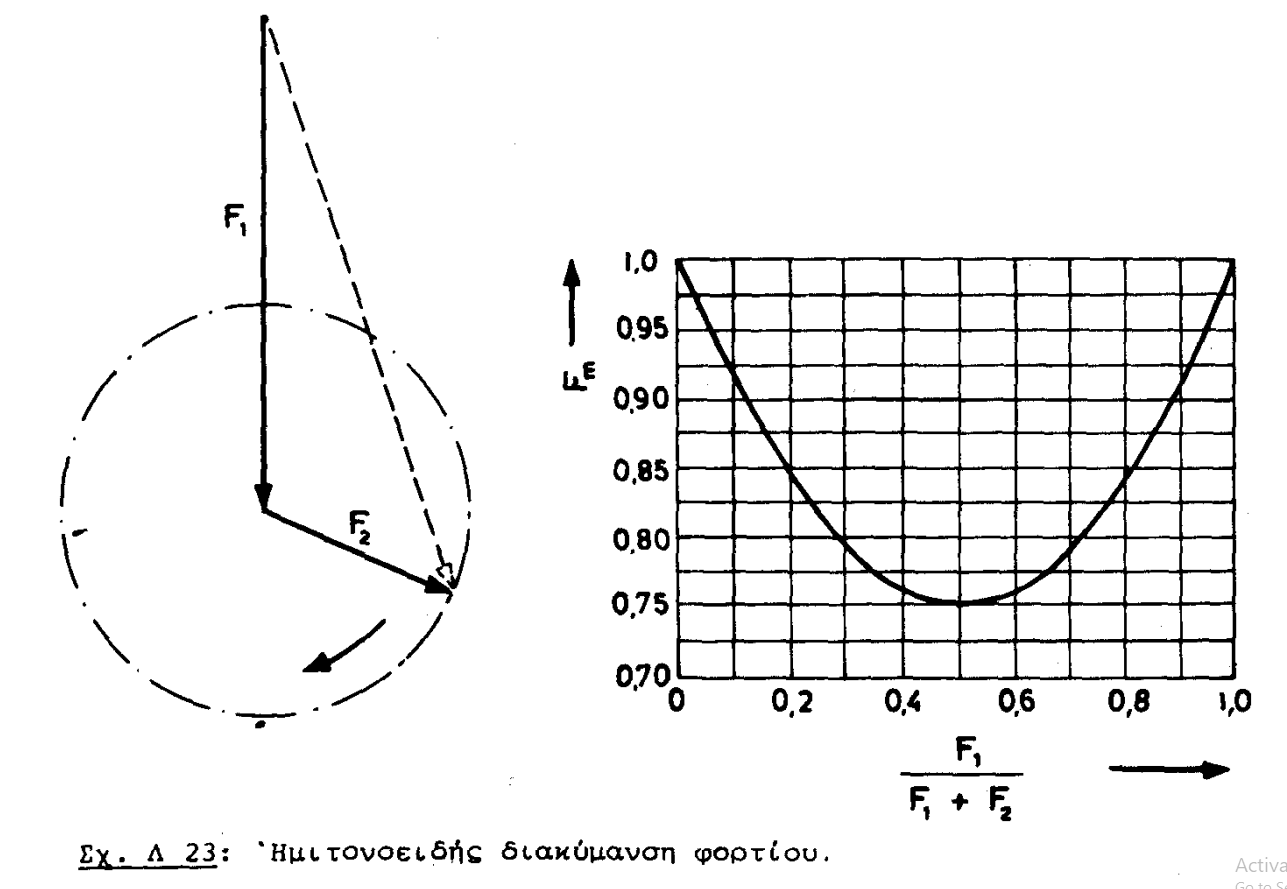
\includegraphics[width=1\linewidth]{3.2.png}
\\
Έπειτα αντικαθιστόυμε όλες τις δυνάμεις που βρίκαμε οτί ασκούνται στο ρουλέμαν (πχ θα τις ονομάσω $A_r$ και $A_x$) με την πραγματική δύναμη $F_r_a_d_i_a_L$ ή $F_a_x_i_a_l$ αντίστοιχα η οποία δίνεται απο τον τύπο:
\\
\begin{center}
    \[ F_r = f_m * A_r * (1+ \frac{\% of fluctuation}{100} \]
\end{center}
\\
Πχ αν $Α_r = 5860$ και για τις αρχικές δυνάνμεις ισχύεουν (πχ $F_U = 1865 +- 30\%$, $F_R = 1713 +- 30\%$, $F_A = 1675 +- 30\%$) και \frac{F1}{F1+F2} = 0.8 τότε:
\\
\[ F_r = 0.85 * 5860 * (1+ \frac{30}{100} \].
    

%%%%%%%%%%%%%%%%%%%%%%%%%%%%%%%%%%%%%%%%%%%%%%%%%%%%%%%%%%%%%%%%%%%%%%%%%%%%%%%%%%%
\section{$C$,$C_o$ (Αριθμός δυναμικής αντοχής,Αριθμός Στατικής αντοχής),\small{(kilopond)}}

Για να βρούμε τον αριθμό δυναμικής αντόχής και τον αριθμό στατικής αντοχής του ρουλεμάν μας πάμε στον Πίνακα Λ27/ΣελΛ137 ο οποίος παρατήθεται παρακάτω και βρίσκουμε τον τύπο του ρουλεμάν που μας δίνει η εκφώνηση. Ο πίνακας αυτός διαβάζεται ως εξής: Αν θέλουμε το ρουλεμάν με αριθμό 6000, τότε θα πάμε στην κατακόρυφη στήλη με τον τίπλο 160(2η στήλη) και θα κατέβουμε μέχρι να βρούμε την γραμμή η οποία έχει τον αριθμό 00(1η γραμμή). Επομένως το ρουλέμαν 6000 έχει $C = 290$ και $C_0 = 156$.
\\
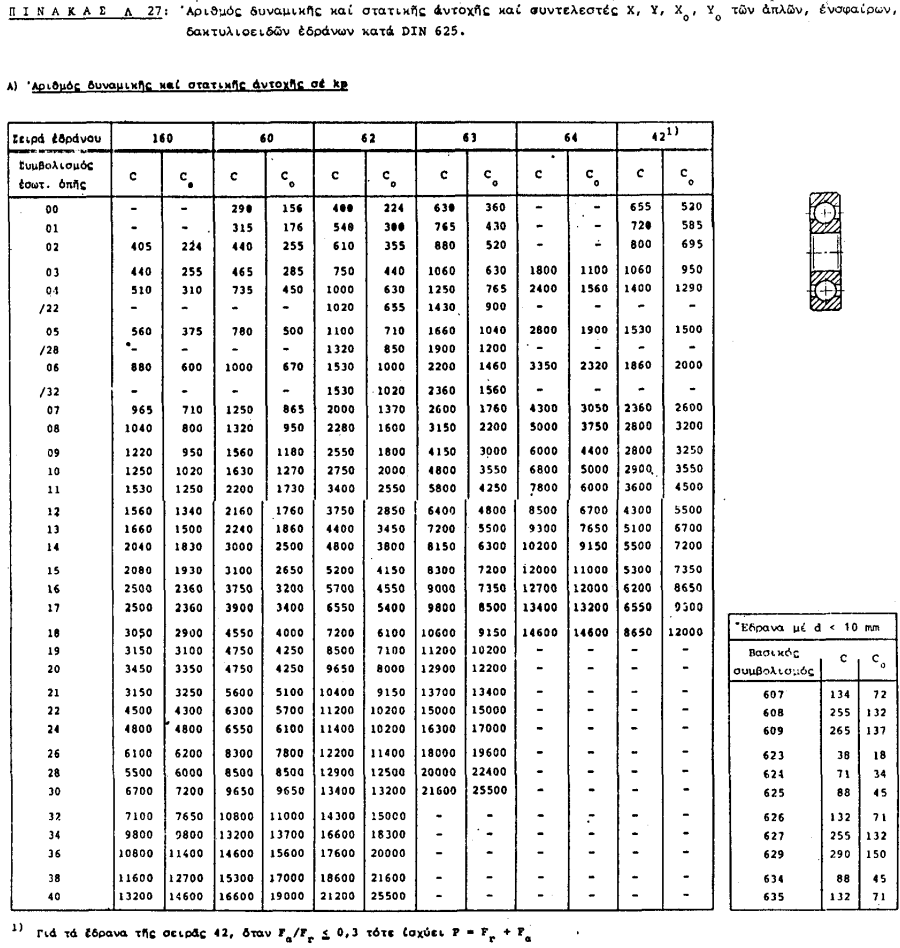
\includegraphics[width=\linewidth]{1.png}
\\

%%%%%%%%%%%%%%%%%%%%%%%%%%%%%%%%%%%%%%%%%%%%%%%%%%%%%%%%%%%%%%%%%%%%%%%%%%%%%%%%%%%%%
\section{$X$,$Υ$ \tiny{(αδιάστατα)}}


Για να βρώ τις τιμές των Χ και Υ πρέπει αρχικά να βρώ την παράμετρο e. Για να βρώ την παράμετρο e πηγαίνω στο πινακάκι Λ27(β)/Σελ Λ137(παρατίθεται παρακάτω) και χρησιμοποιώντας το πυλίκο \textbf{$\frac{F_a}{C_0}$} βρίσω την τιμή e στην οποία αντιχτοιχεί. \textbf{Αν δεν υπάρχει ακριβής αντιστοίχηση κάνω γραμμική παρεμβολή.} 
\\
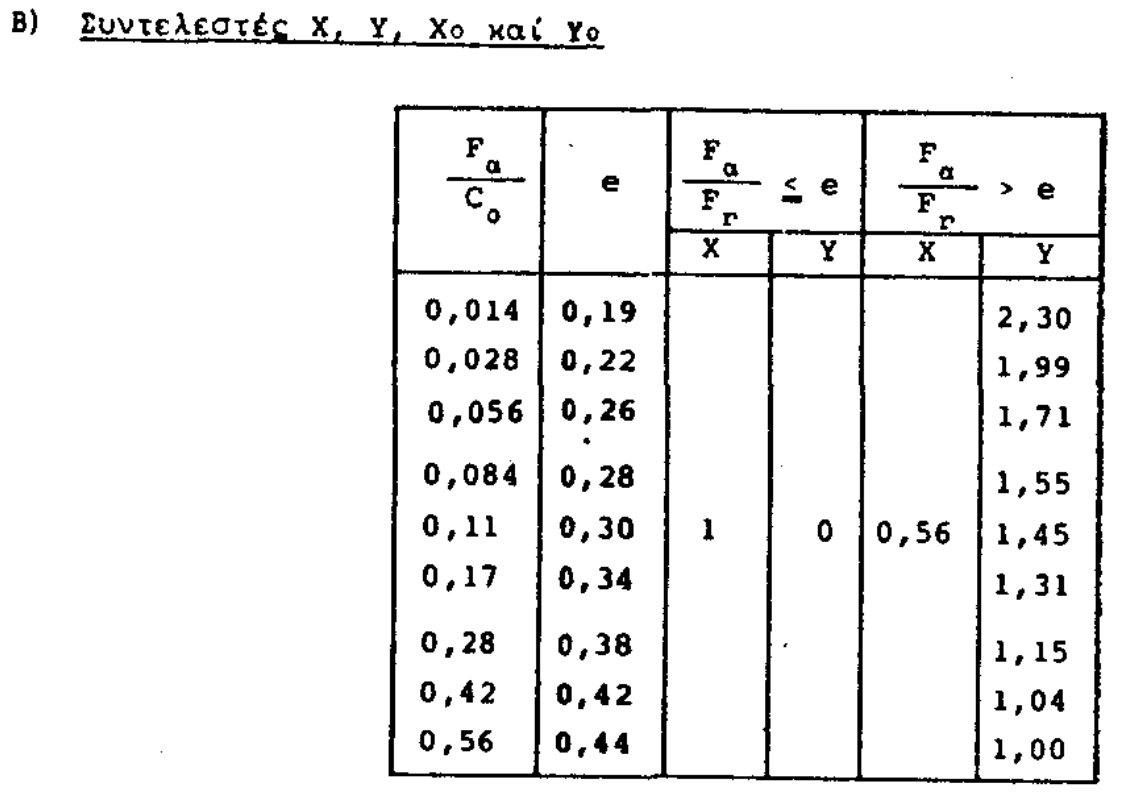
\includegraphics[width=\linewidth]{2.png}
\\Έπειτα βρίσκω τα X και Y ανάλογα με το ποιά συνθήκη ισχύει($\frac{F_a}{C_0} < e$ ή $\frac{F_a}{C_0} > e$. Αν ισχύει η δέυτερη συνθήκη τότε κάνω γραμική παρεμβολή ανάμεσα στις τιμές του e και του Y.

%%%%%%%%%%%%%%%%%%%%%%%%%%%%%%%%%%%%%%%%%%%%%%%%%%%%%%%%%%%%%%%%%%%%%%%%%%%%%%%%%%%%%
\section{$P$ (Ισοδύναμο φορτίο) \tiny{(kilopond)}}
Για να βρώ το ισοδύναμο φορτίο χρησιμοποιώ τον παρακάτω τύπο.
\begin{center}
    \[ P = X*F_r + Y*F_a \]
\end{center}
\\


%%%%%%%%%%%%%%%%%%%%%%%%%%%%%%%%%%%%%%%%%%%%%%%%%%%%%%%%%%%%%%%%%%%%%%%%%%%%%%%%
\section{$L_h$ (Ώρες Λειτουργίας)}
Ισχύει οτι:
\begin{center}
    \[ L_h = \frac{10^6}{60*n}*\frac{C}{P}^k \]
\end{center}
\\
Όπου:
\begin{itemize}
    \item k = 3 για ένσφαιρα έδρανα κυλήσεως
    \item k = 10/3 για το υπόλοιπα έιδη έδράνων κυλίσεως
\end{itemize}

%%%%%%%%%%%%%%%%%%%%%%%%%%%%%%%%%%%%%%%%%%%%%%%%%%%%%%%%%%%%%%%%%%%%%%%%%%%%%%%%%
\section{Πίνακες Ρουλεμάν}
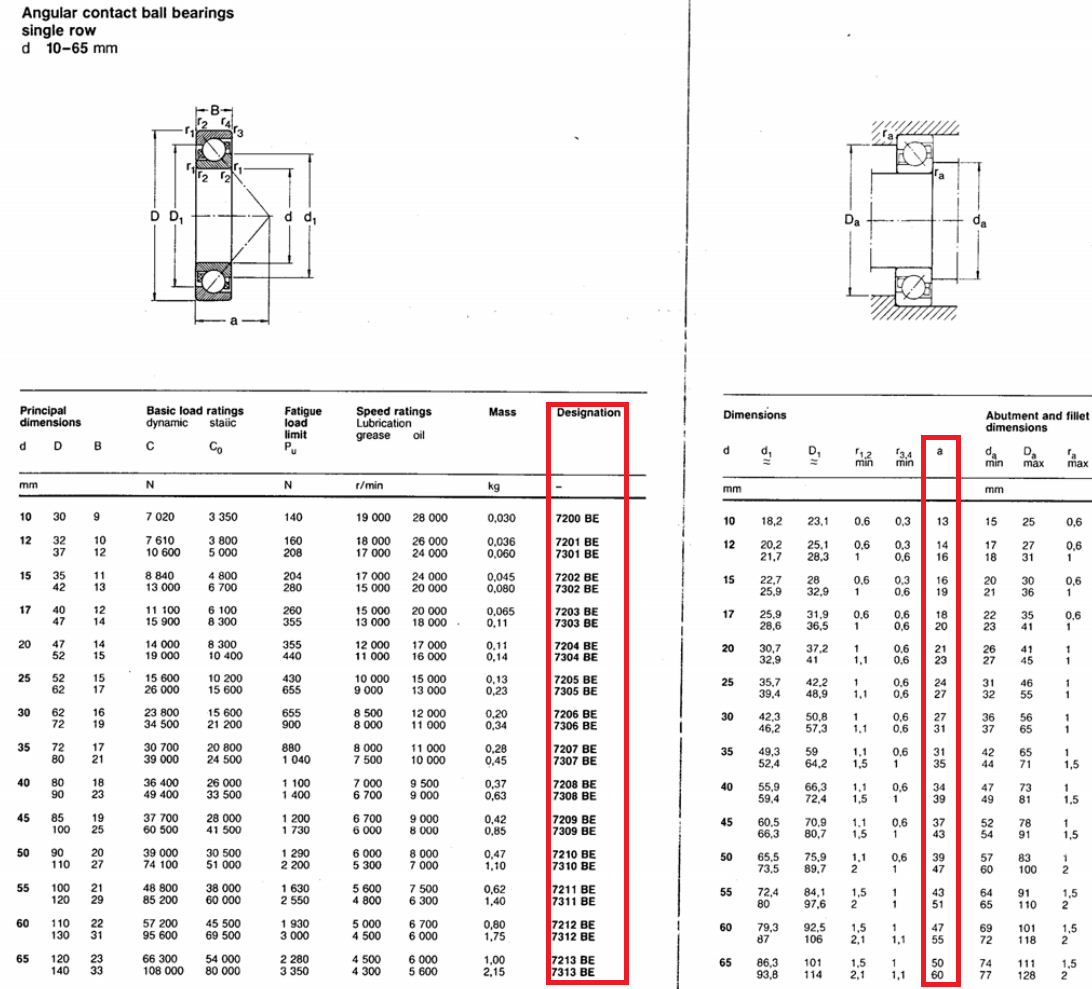
\includegraphics[width=0.9\linewidth]{4.png}
\\
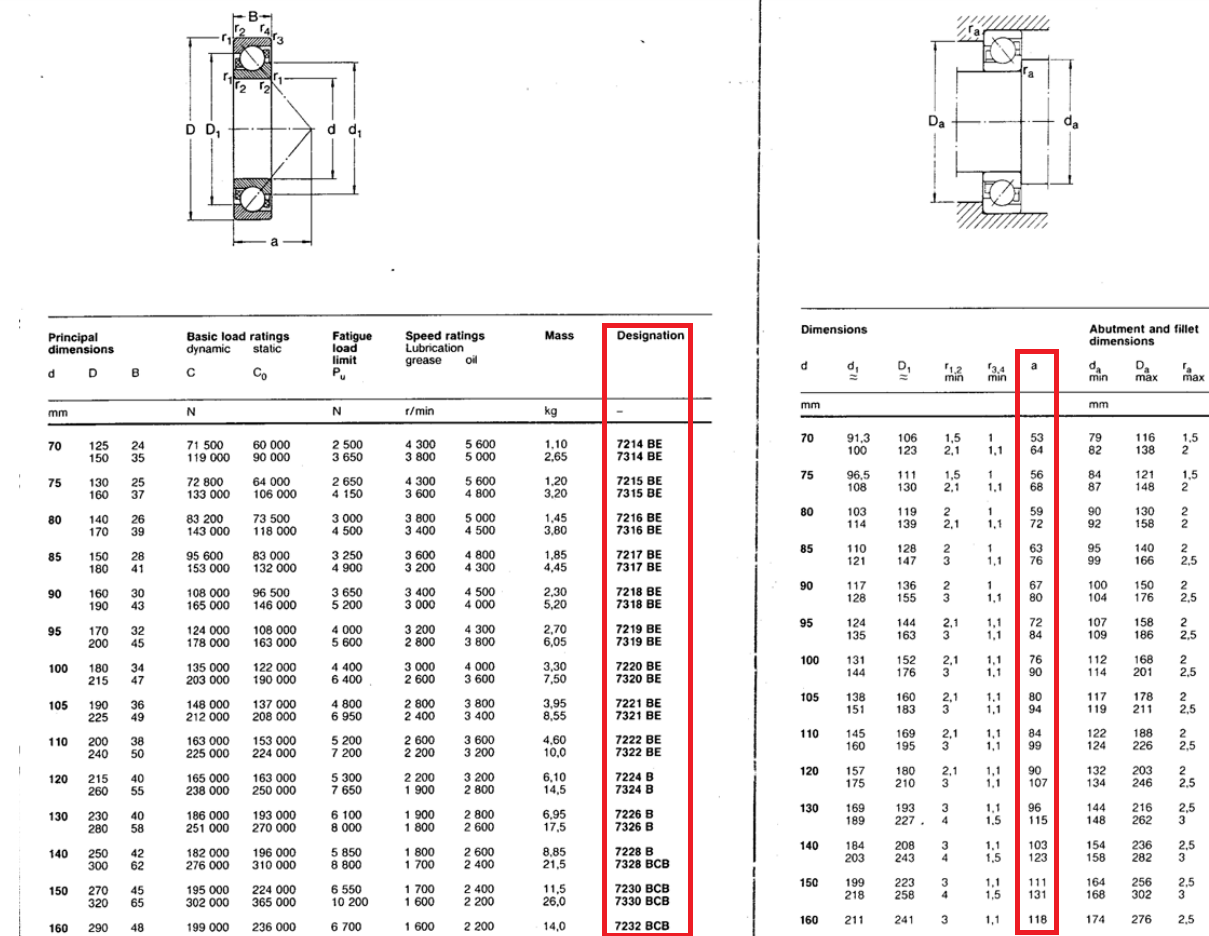
\includegraphics[width=0.9\linewidth]{5.png}
\\
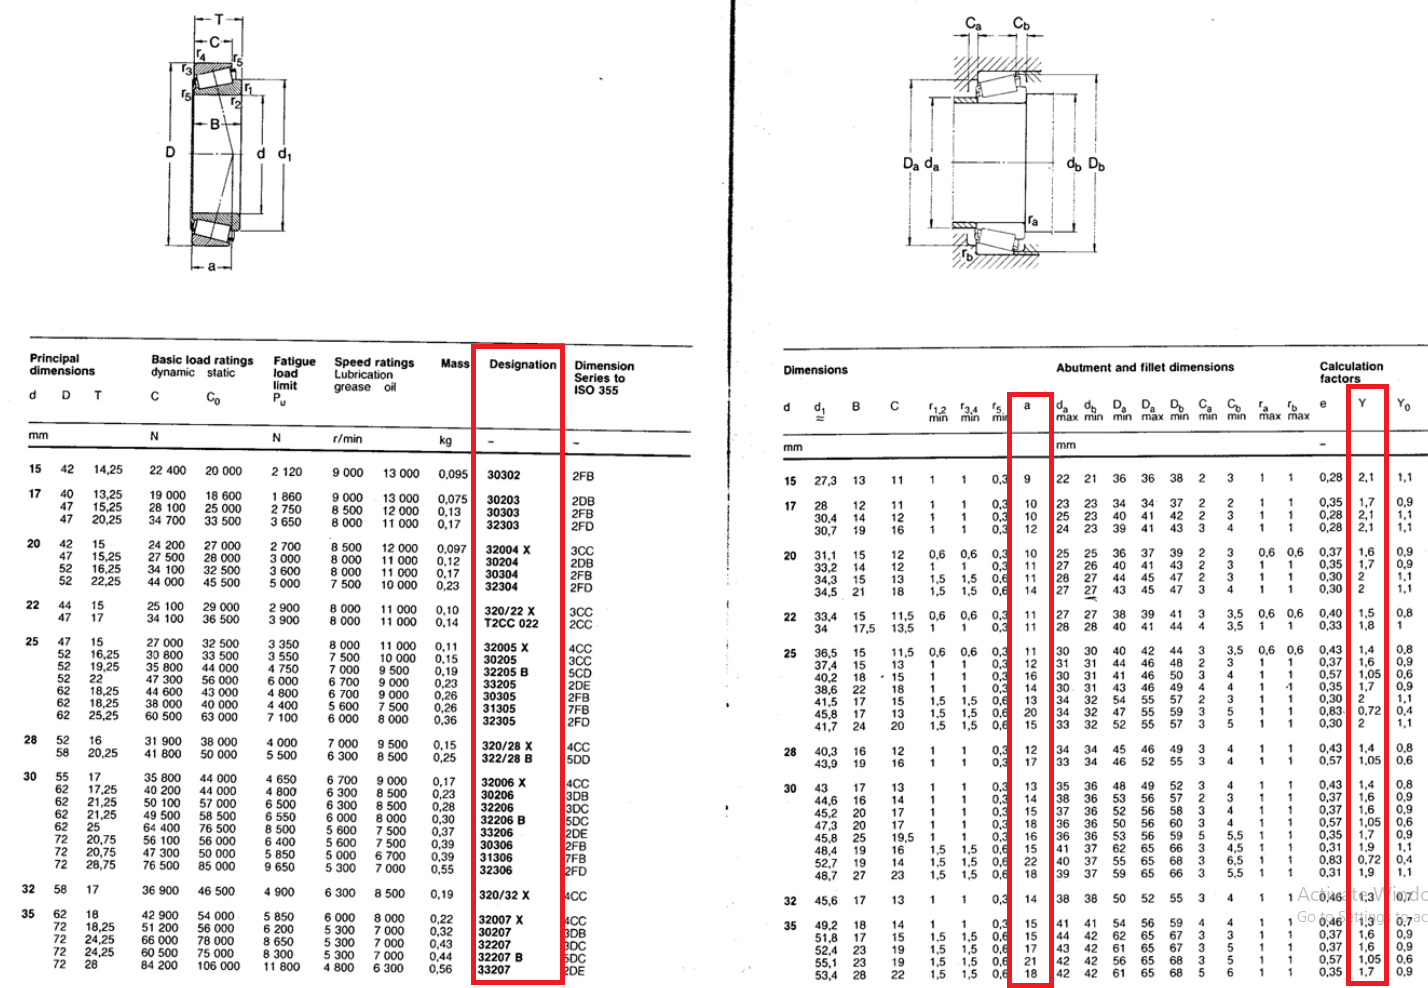
\includegraphics[width=0.9\linewidth]{6.png}
\\
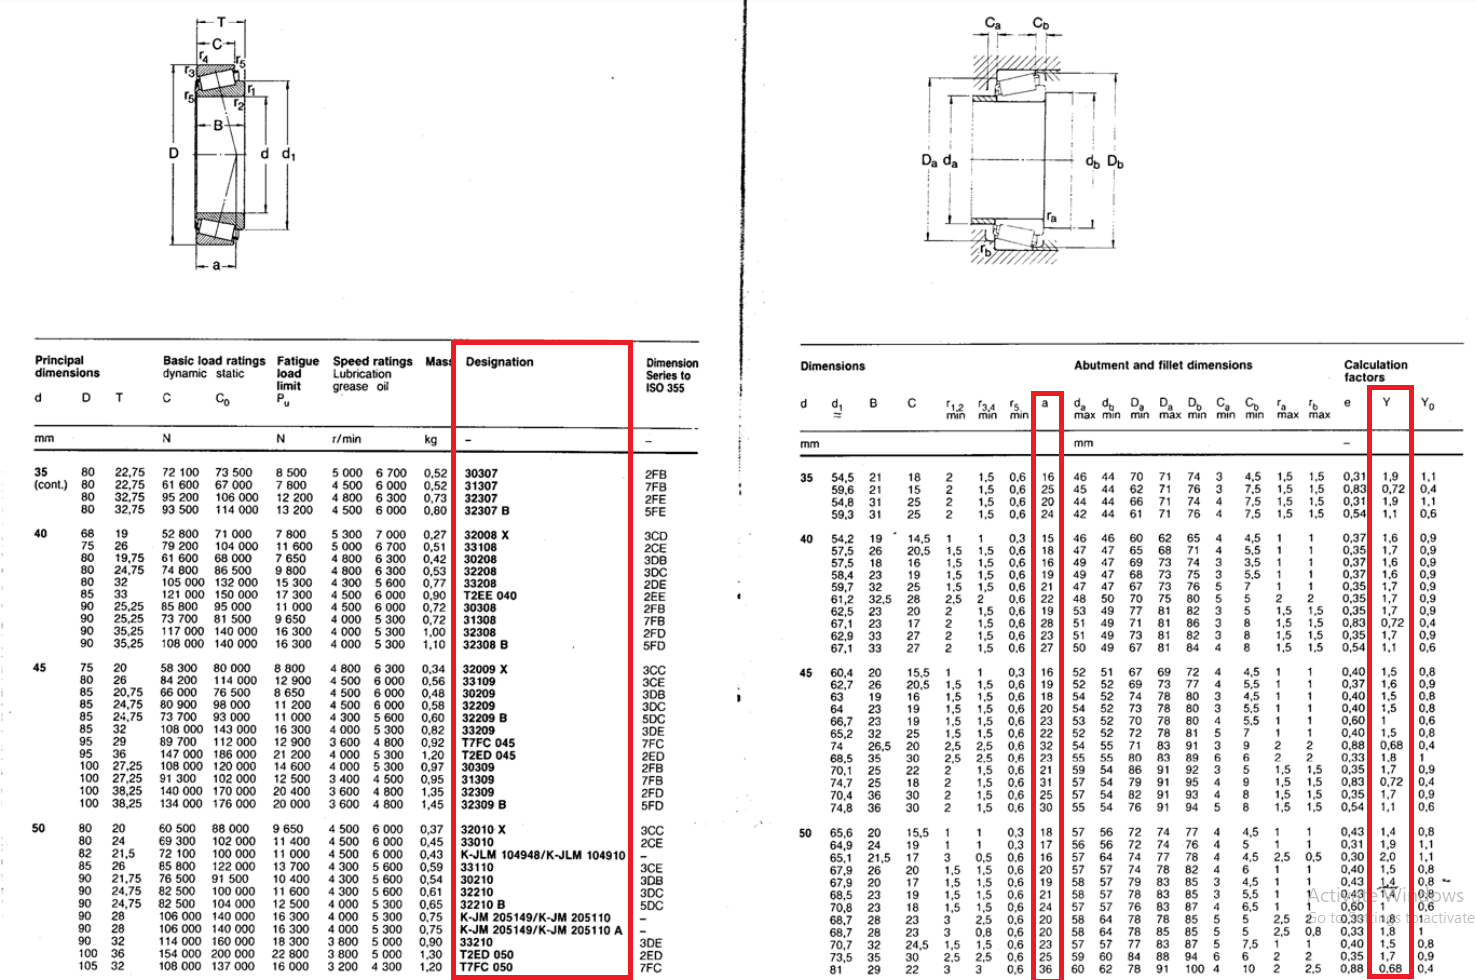
\includegraphics[width=0.9\linewidth]{7.png}
\\
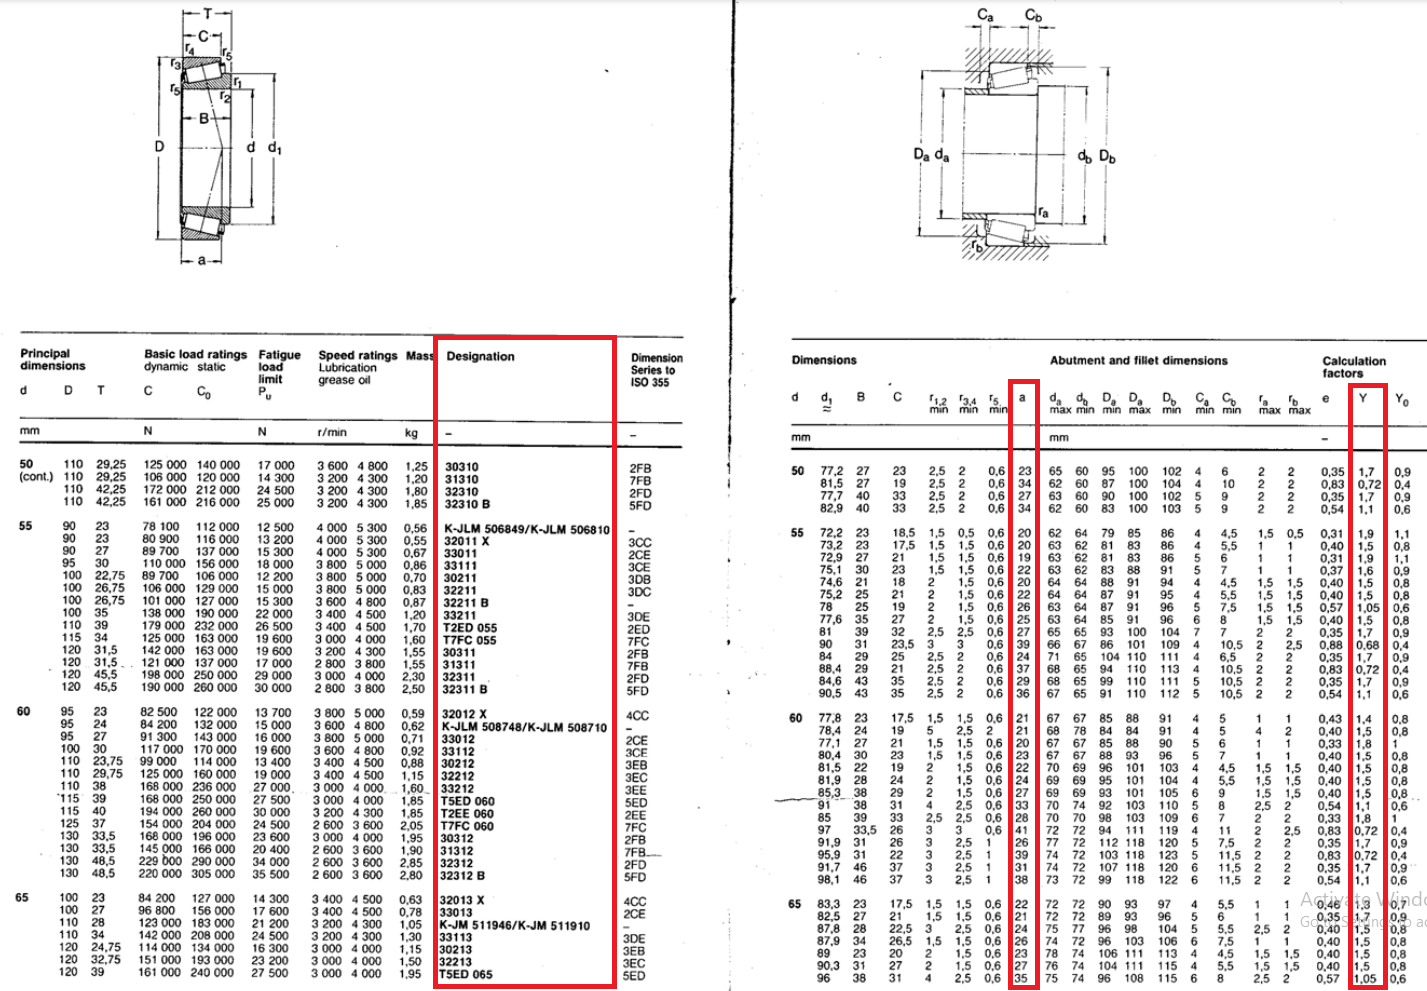
\includegraphics[width=0.9\linewidth]{8.png}
\\
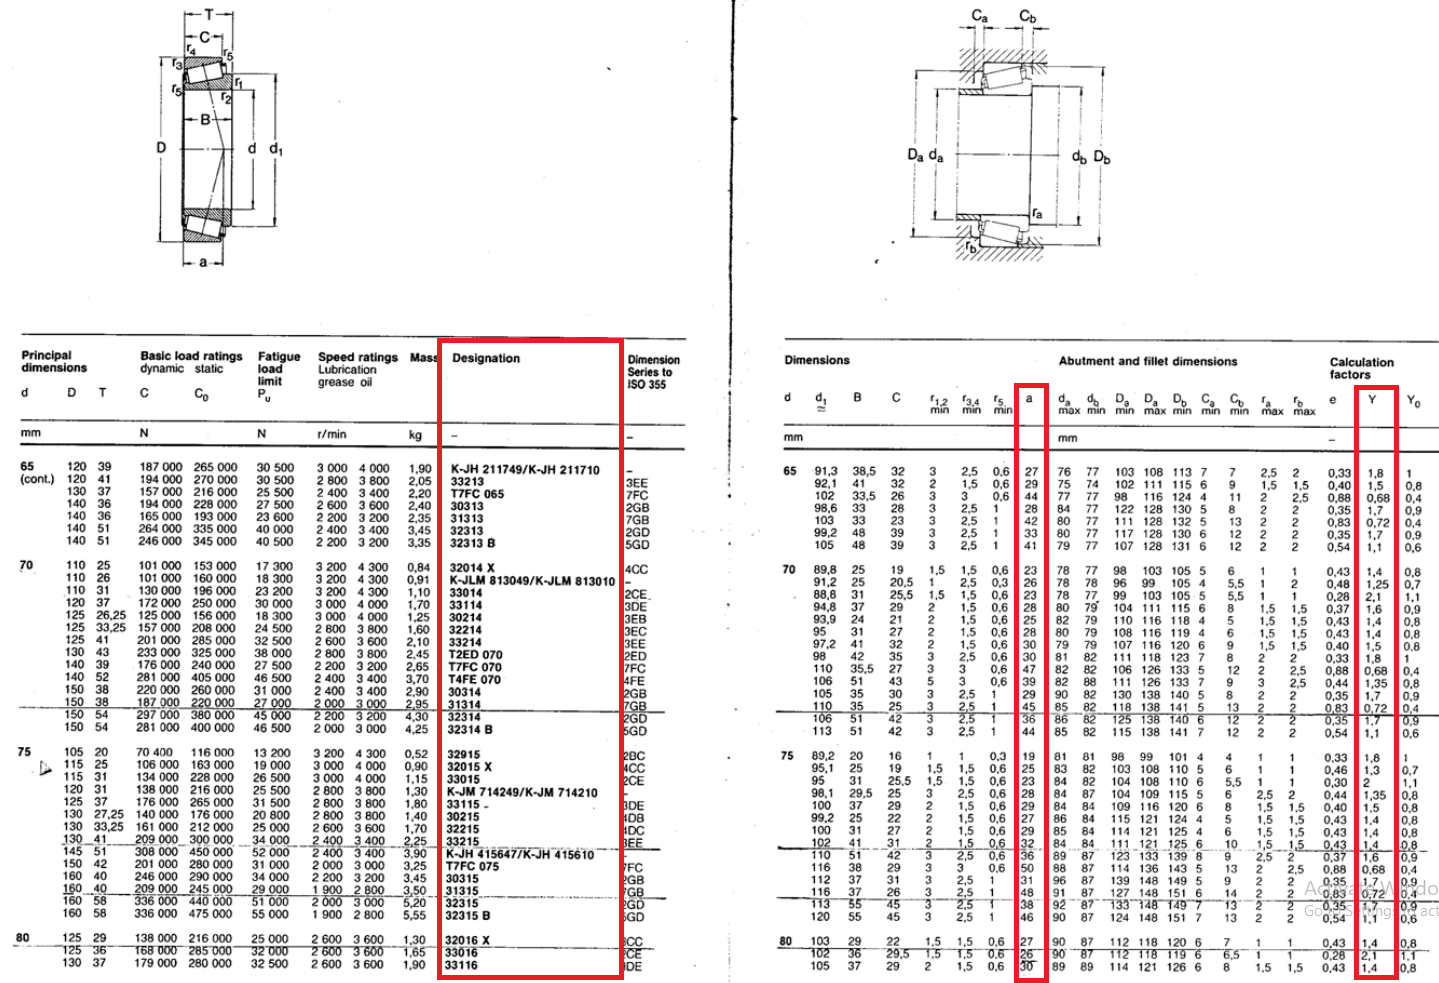
\includegraphics[width=0.9\linewidth]{9.png}
\\
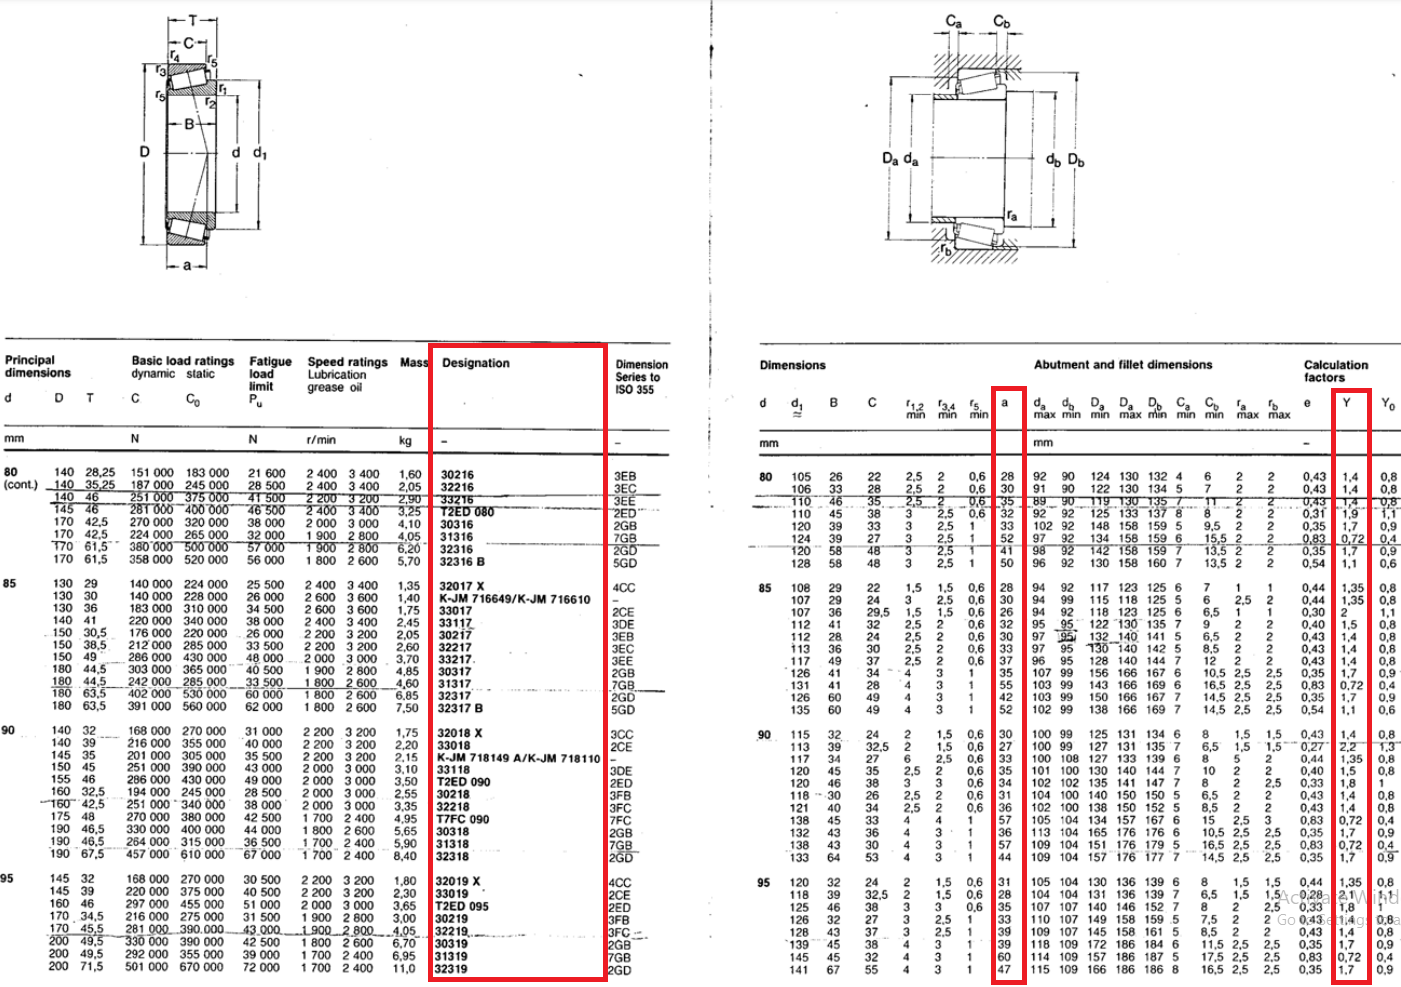
\includegraphics[width=0.9\linewidth]{10.png}

\end{document}